\documentclass{article}
\usepackage{tikz}
\usetikzlibrary{arrows.meta,positioning,calc,shapes.geometric}
\pagestyle{empty}
\begin{document}
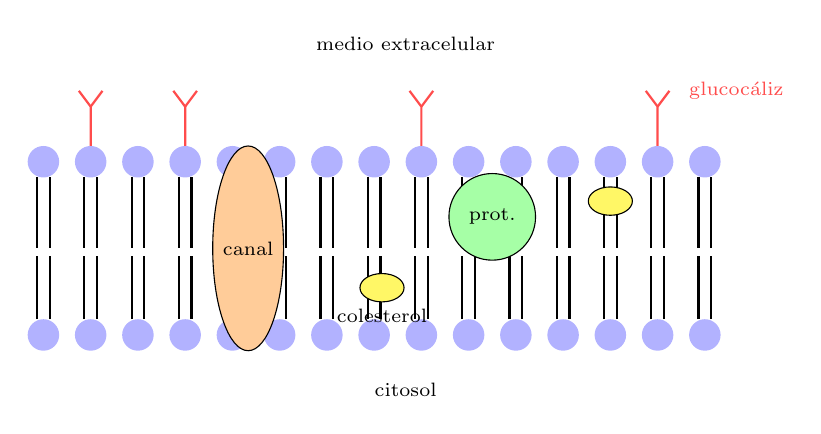
\begin{tikzpicture}

\foreach \x in {0.4,1.0,...,9.4} {
  \fill[blue!30] (\x,2.2) circle (0.2); \draw[thick] (\x-0.08,2.0) -- (\x-0.08,1.1); \draw[thick] (\x+0.08,2.0) -- (\x+0.08,1.1);
  \fill[blue!30] (\x,0.0) circle (0.2); \draw[thick] (\x-0.08,0.2) -- (\x-0.08,1.0); \draw[thick] (\x+0.08,0.2) -- (\x+0.08,1.0);
}
\draw[fill=orange!40] (3.0,1.1) ellipse (0.45 and 1.3); \node[font=\scriptsize] at (3.0,1.1) {canal};
\draw[fill=green!35] (6.1,1.5) ellipse (0.55 and 0.55); \node[font=\scriptsize] at (6.1,1.5) {prot.};
\draw[fill=yellow!60] (4.7,0.6) ellipse (0.28 and 0.18); \draw[fill=yellow!60] (7.6,1.7) ellipse (0.28 and 0.18); \node[font=\scriptsize] at (4.7,0.25) {colesterol};
\foreach \x in {1.0,2.2,5.2,8.2} {\draw[red!70, thick] (\x,2.4) -- (\x,2.9) -- (\x-0.15,3.1); \draw[red!70, thick] (\x,2.9) -- (\x+0.15,3.1);}
\node[font=\scriptsize, red!70] at (9.2,3.1) {glucocáliz};
\node[font=\scriptsize] at (5,-0.7) {citosol}; \node[font=\scriptsize] at (5,3.7) {medio extracelular};

\end{tikzpicture}
\end{document}
